\documentclass{beamer}
\usetheme{CambridgeUS}
\usecolortheme{beaver}

\newcommand\hmmax{0}
\newcommand\bmmax{0}

\usepackage{stmaryrd}

\usepackage{amsmath,amssymb,enumerate,amsthm}
\usepackage{bm}
\usepackage{graphicx}

\usepackage{algorithm, algpseudocode}
\usepackage[strict]{siunitx}
\usepackage{hyperref}
\usepackage{mathrsfs}

\usepackage{bm}
\usepackage{empheq}
\usepackage{cleveref}
\usepackage{xcolor}
\usepackage{textcomp}

\NewDocumentCommand{\R}{}{\mathbb{R}}
\NewDocumentCommand{\N}{}{\mathbb{N}}
%\mathscr is rounder than \mathcal.
\NewDocumentCommand{\powerset}{m}{\mathscr{P}(#1)}
%Powerset without zero.
\NewDocumentCommand{\powersetz}{m}{\mathscr{P}^*(#1)}
%https://tex.stackexchange.com/a/45732, works within both \set and \set*, same spacing than \mid (https://tex.stackexchange.com/a/52905).
\NewDocumentCommand{\suchthat}{}{\;\ifnum\currentgrouptype=16 \middle\fi|\;}
%Integer interval.
\NewDocumentCommand{\intvl}{m}{\llbracket#1\rrbracket}
%Allows for \abs and \abs*, which resizes the delimiters.
\DeclarePairedDelimiter\abs{\lvert}{\rvert}
\DeclarePairedDelimiter\card{\lvert}{\rvert}
\DeclarePairedDelimiter\floor{\lfloor}{\rfloor}
\DeclarePairedDelimiter\ceil{\lceil}{\rceil}
%Perhaps should use U+2016 ‖ DOUBLE VERTICAL LINE here?
\DeclarePairedDelimiter\norm{\lVert}{\rVert}
%From mathtools. Better than using the package braket because braket introduces possibly undesirable space. Then: \begin{equation}\set*{x \in \R^2 \suchthat \norm{x}<5}\end{equation}.
\DeclarePairedDelimiter\set{\{}{\}}
\DeclareMathOperator*{\argmax}{arg\,max}
\DeclareMathOperator*{\argmin}{arg\,min}

%UTR #25: Unicode support for mathematics recommend to use the straight form of phi (by default, given by \phi) rather than the curly one (by default, given by \varphi), and thus use \phi for the mathematical symbol and not \varphi. I however prefer the curly form because the straight form is too easy to mix up with the symbol for empty set.
\let\phi\varphi

%The amssymb solution.
%\NewDocumentCommand{\restr}{mm}{{#1}_{\restriction #2}}
%Another acceptable solution.
%\NewDocumentCommand{\restr}{mm}{{#1|}_{#2}}
%https://tex.stackexchange.com/a/278631; drawback being that sometimes the text collides with the line below.
\NewDocumentCommand\restr{mm}{#1\raisebox{-.5ex}{$|$}_{#2}}


%Decision Theory (MCDA and SC)
\NewDocumentCommand{\allalts}{}{\mathcal{A}}
\NewDocumentCommand{\allcrits}{}{\mathscr{C}}
\NewDocumentCommand{\alts}{}{A}
\NewDocumentCommand{\dm}{}{i}
\NewDocumentCommand{\allF}{}{\mathscr{F}}
\NewDocumentCommand{\allvoters}{}{\mathcal{N}}
\NewDocumentCommand{\voters}{}{N}
\NewDocumentCommand{\prof}{}{P}
\NewDocumentCommand{\linors}{}{\mathcal{L}(\allalts)}
\NewDocumentCommand{\alllosses}{}{\intvl{0, m-1}^N}
%Thanks to https://tex.stackexchange.com/q/154549
	%\makeatletter
	%\def\@myRgood@#1#2{\mathrel{R^X_{#2}}}
	%\def\myRgood{\@ifnextchar_{\@myRgood@}{\mathrel{R^X}}}
	%\makeatother
\NewDocumentCommand{\pref}{}{\succ}
\NewDocumentCommand{\prefi}{O{i}}{\succ_{#1}}
\NewDocumentCommand{\PO}{}{\mathit{PO}}

%Deliberated Judgment
\NewDocumentCommand{\allargs}{}{S^*}
\NewDocumentCommand{\args}{}{S}
\NewDocumentCommand{\ar}{}{s}
\NewDocumentCommand{\allprops}{}{T}
\NewDocumentCommand{\prop}{}{t}
\NewDocumentCommand{\ileadsto}{}{⇝}
\NewDocumentCommand{\ibeatse}{}{⊳_\exists}
\NewDocumentCommand{\nibeatse}{}{⋫_\exists}
\NewDocumentCommand{\ibeatsst}{}{⊳_\forall}
\NewDocumentCommand{\nibeatsst}{}{⋫_\forall}
\NewDocumentCommand{\mleadsto}{O{\eta}}{⇝_{#1}}
\NewDocumentCommand{\mbeats}{O{\eta}}{⊳_{#1}}
\NewDocumentCommand{\ibeatseinv}{}{⊳_\exists^{-1}}

%Logic
\NewDocumentCommand{\ltru}{}{\texttt{T}}
\NewDocumentCommand{\lfal}{}{\texttt{F}}
\newtheorem{remark}{Remark}


\newcommand{\profile}{\bm{v}}%(complete) profile
\newcommand{\pprofile}{{\bm{p}}}%partial profile
\newcommand{\w}{\bm{w}}
\newcommand{\W}{\mathcal{W}}
\newcommand{\Co}{\mathcal{C}}
\newcommand{\pw}{W}%our knowledge about the weights
\newcommand{\strat}[1]{\emph{#1}}
\newcommand{\ppref}{\succ^\text{p}}%partial pref
\newcommand{\pprefeq}{\succeq^\text{p}}%partial pref
\DeclareMathOperator{\Regret}{Regret}
\DeclareMathOperator{\SCORE}{Score}
\DeclareMathOperator{\PMR}{PMR}
\DeclareMathOperator{\MR}{MR}
\DeclareMathOperator{\MMR}{MMR}

\newcommand*{\icimg}[1]{%
	\raisebox{-.3\baselineskip}{%
		\includegraphics[
		height=\baselineskip,
		width=\baselineskip,
		keepaspectratio,
		]{#1}%
	}%
}

\newcommand*{\icarr}[1]{%
	\raisebox{-0.4\baselineskip}{%
		\includegraphics[
		height=2.5\baselineskip,
		width=3\baselineskip,
		keepaspectratio,
		]{#1}%
	}%
}

\makeatletter
\defbeamertemplate*{title page}{mydefault}[1][]
{
	\vbox{}
	\vfill
	\begin{centering}

%{\usebeamercolor[fg]{titlegraphic}\inserttitlegraphic\par}
		\begin{beamercolorbox}{titlegraphic}
				\usebeamerfont{titlegraphic}\inserttitlegraphic
		\end{beamercolorbox}%
			\vskip1em\par	
		\begin{beamercolorbox}[rounded=true, center, shadow=true, sep=8pt,#1]{title}
			\usebeamerfont{title}\inserttitle\par%
			\ifx\insertsubtitle\@empty%
			\else%
			\vskip0.5em%
			{\usebeamerfont{subtitle}\usebeamercolor[fg]{subtitle}\insertsubtitle\par}%
			\fi%     
		\end{beamercolorbox}%
		\vskip1em\par
		\begin{beamercolorbox}[sep=8pt,center,#1]{author}
			\usebeamerfont{author}\insertauthor
		\end{beamercolorbox}
		\begin{beamercolorbox}[sep=8pt,center,#1]{institute}
			\usebeamerfont{institute}\insertinstitute
		\end{beamercolorbox}
		\begin{beamercolorbox}[sep=8pt,center,#1]{date}
			\usebeamerfont{date}\insertdate
		\end{beamercolorbox}\vskip0.5em
		\begin{beamercolorbox}[sep=8pt,center,#1]{logo}
			\usebeamerfont{titlegraphic}\insertlogo
		\end{beamercolorbox}%
	\end{centering}
	\vfill
}
\setbeamertemplate{title page}[mydefault]
\makeatother



\titlegraphic{
\includegraphics[width=50mm]{logo_dauphine} \hspace*{5.5cm} 
\includegraphics[width=7mm]{cnrs}}
\title[Elicitation and explanation for voting rules]{Elicitation and explanation for voting rules}
%\subtitle{Proposal: ``Elicitation and Explanation for Voting Rules''}
\author[Beatrice Napolitano]{\textbf{Beatrice Napolitano} \\
	Supervisors: Remzi Sanver, Olivier Cailloux}
\date[06 July 2021]{ Pré-soutenance de thèse \\ 06 July 2021 \\ 
\includegraphics[width=35mm]{LOGO_LAMSADE} }

\usepackage{tikz}
\usepackage{amsmath}
\usepackage{graphicx}

\definecolor{darkred}{rgb}{0.8,0,0}

\begin{document}

\beamertemplatenavigationsymbolsempty

\begin{frame}[plain]
\maketitle
\end{frame}

\addtocounter{framenumber}{-1}

\begin{frame}
	\frametitle{Outline}
	\tableofcontents[hideallsubsections, sectionstyle=shaded/show]
\end{frame}

\AtBeginSection{
	\begin{frame}
		\frametitle{Outline}
		\tableofcontents[currentsection, hideallsubsections]
	\end{frame}
}

\section{Notation}
\subsection{Context}
\begin{frame}
	\frametitle{Context}	
	\begin{description}[$f: \linors^\voters \rightarrow \powersetz{\allalts}$]
		\item [$\allalts$] alternatives, $|\allalts|=m$
		\item [$\voters$] voters, $|\voters|=n$
		\item [$\linors$, ${\prefi} \in \linors$] a linear order over $\allalts$
		\item [$\prof \in \linors^\voters$] a profile
		\item [$\powersetz{\allalts}$] the possible winners (the non-empty subsets of $\allalts$)
		\item [$f: \linors^\voters \rightarrow \powersetz{\allalts}$] a SCR
	\end{description}
\end{frame}

\section{Compromising as an equal loss principle}
\subsection{Context}
\begin{frame}
	\frametitle{Context}
	\framesubtitle{Introducing the problem}
	\textbf{Setting}: Several voters express their preferences over a set of alternatives \vspace{6mm}
	
	\onslide<2->{\textbf{Goal}: Find a procedure determining a collective choice that promotes a notion of compromise}
\end{frame}

\subsection{Related Works}
\begin{frame}
	\frametitle{Context}
	\framesubtitle{Related Works}
	\begin{itemize}
		\item<1-> \textbf{Plurality}: selects the alternatives considered as best by the highest number of voters 
		%	In other words, it insists on a support of first and highest quality, disregarding the quantity of support this may lead to.
		\item<2-> \textbf{Median Voting Rule}: picks all alternatives receiving a majority of support at the highest possible quality
		\item<3-> \textbf{Majoritarian Compromise}: MVR and ties are broken according to the quantity of support these receive
		%gives up from the quality of support, in order to ensure a majority support behind the selected alternatives.
		\item<4-> \textbf{Fallback Bargaining}: bargainers fall back to less and less preferred alternatives until they reach a unanimous agreement 
		\item<5-> \textbf{q-approval FB}: picks the alternatives which receive the support of q voters at the highest possible quality, breaking ties according to the quantity of support
		%	Note that MC and FB winners are	particular cases of q-approval compromises, for q being respectively equal to majority and unanimity. Moreover for q = 1, q-approval compromises	coincide with the plurality rule (PR) winners
	\end{itemize}
\end{frame}

\begin{frame}
	\frametitle{Context}
	\framesubtitle{Motivation: A simple example}
	$n=100, \allalts=\{a,b,c\}$
	\begin{center}
		$
		\begin{array}{cccc}
			\mathbf{51} \quad &a&b&c\\
			\mathbf{49} \quad &c&b&a\\
		\end{array}
		$
	\end{center}
	\begin{itemize}
		\item<2-> Plurality: $\{a\}$
		\item<3-> MVR: $\{a\}$
		\item<4-> MC: $\{a\}$
		\item<5-> FB: $\{b\}$
		\item<6-> q-approval FB 	$q\in \left\{ 1,..., \frac{n}{2} +1\right\} $: $\{a\}$
	\end{itemize}
	\vspace{0.5cm}
	\visible<7->{\centering Does $b$ seem a better compromise?}
\end{frame}

\begin{frame}
	\frametitle{Notation}
	%Our compromises attempt to equalize “losses”
	\begin{description}[$\lambda_{\prof}: \allalts \rightarrow \intvl{0, m - 1}^\voters$]
		\item<1-> [$\lambda_{\prof}: \allalts \rightarrow \intvl{0, m - 1}^\voters$] a loss vector
	\end{description}
	\vspace{4cm} 
	%Thus, the spread of $l$ gets its lowest value $0$ in case of perfect equality and only in this case.
\end{frame}

\begin{frame}
	\frametitle{Notation}
	\framesubtitle{Losses}
		\begin{center}
		\begin{tikzpicture}
			\path node (P) {$\prof$};
			\path (P.south) node[anchor=north] (profile) {$%
				\begin{array}{r@{\hspace{1mm} : \hspace{1mm}}l}
					v_1 & a \pref b \pref c\\%
					v_2 & c \pref b \pref a\\%
				\end{array}%
				$};
			\path (P.center) ++ (3cm, 0) node (L) {$\lambda_{\prof}$};
			\path (L.south) node[anchor=north] (losses) {$%
				\begin{array}{r@{\hspace{1mm} : \hspace{1mm}}l}
					a & (0, 2)\\%
					b & (1, 1)\\%
					c & (2, 0)\\%
				\end{array}%
				$};
		\end{tikzpicture}
		\end{center}
	\bigskip
	
	Given $\prof = (\prefi)_{i \in N}$:
	\begin{itemize}
		\item $\lambda_{\prefi}(x) = \card{\set{y \in \allalts \suchthat y \prefi x}} \in \intvl{0, m - 1}$ the loss of $i$ when choosing $x \in \allalts$ instead of her favorite alternative
		\item $\lambda_{\prof}(x)$ associates to each voter her loss when choosing $x$
	\end{itemize}
\end{frame}

\begin{frame}
	\frametitle{Notation}
	%Our compromises attempt to equalize “losses”
	\begin{description}[$\lambda_{\prof}: \allalts \rightarrow \intvl{0, m - 1}^\voters$]
		\item<1-> [$\lambda_{\prof}: \allalts \rightarrow \intvl{0, m - 1}^\voters$] a loss vector
		\item<2-> [$\sigma: \intvl{0, m - 1}^N \rightarrow \R^+$] a spread measure
	\end{description}
	\bigskip
	\onslide<3-> \begin{block}{}
		$\Sigma$ is the set of spread measures $\sigma$ such that 
		\[ \sigma(l)=0 \iff l_{i}=l_{j}, \ \forall i,j\in N, \quad \forall l\in\alllosses \].
	\end{block}
	%Thus, the spread of $l$ gets its lowest value $0$ in case of perfect equality and only in this case.
\end{frame}

\section[Simultaneous Elicitation of PSR and Agent Preferences]{Simultaneous Elicitation of Scoring Rule and Agent Preferences for Robust Winner Determination}

\begin{frame}[t]
	\frametitle{Classical Scenario}
	\textbf{Setting}: Voters specify preferences over alternatives and a committee defines the social choice rule to aggregate them
	\begin{figure}
		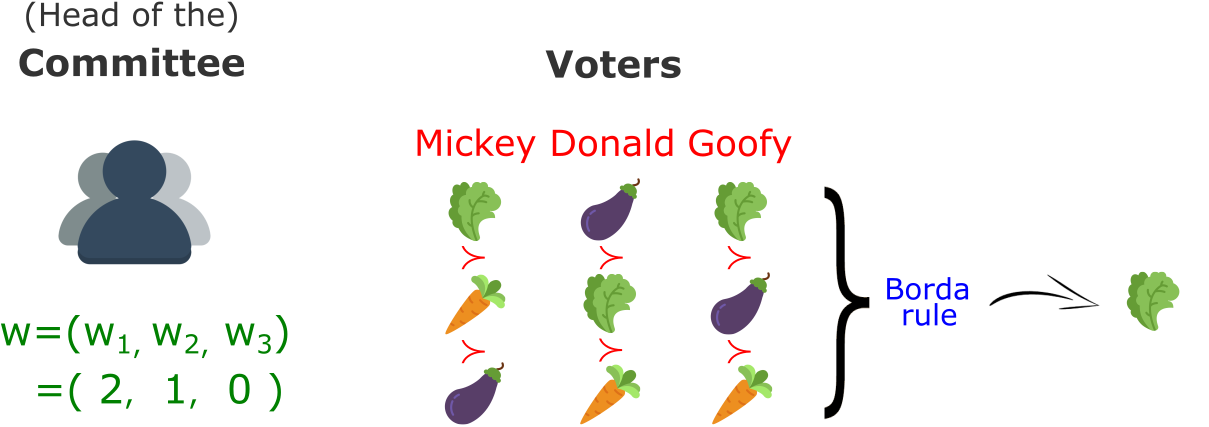
\includegraphics[scale=0.35]{classset.png}
		%		\caption{.}
		%		\label{fig:b1}
	\end{figure}
	\onslide<2-> \textbf{Goal}: Find a consensus choice 
\end{frame}


\section{Setting}
\subsection{Scenario}

\begin{frame}[t]
	\frametitle{Classical Scenario}
	\textbf{Setting}: Voters specify preferences over alternatives and a committee defines the social choice rule to aggregate them
	\begin{figure}
		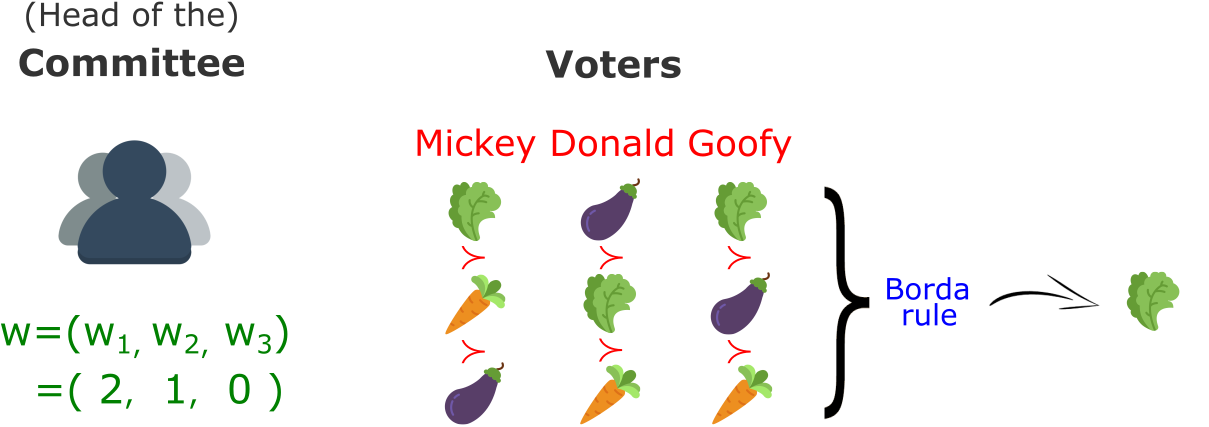
\includegraphics[scale=0.35]{classset.png}
		%		\caption{.}
		%		\label{fig:b1}
	\end{figure}
	\onslide<2-> \textbf{Goal}: Find a consensus choice 
\end{frame}

\begin{frame}[t]
\frametitle{Our Scenario}
%\framesubtitle{Robust Winner Determination}
%	\textbf{Setting}: Two kind of players
\textbf{Setting}: Incompletely specified preferences and social choice rule \bigskip
\begin{figure}
	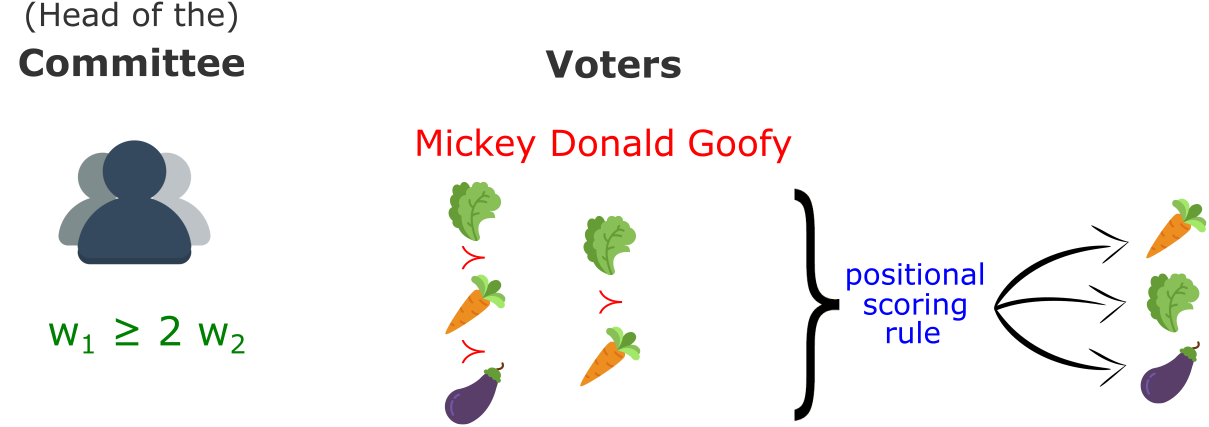
\includegraphics[scale=0.35]{ourset.png}
	%		\caption{.}
	%		\label{fig:b1}
\end{figure}
\onslide<2-> \textbf{Goal}: Develop an incremental elicitation strategy to acquire the most relevant information 
\end{frame}
%\addtocounter{framenumber}{-1}
%\begin{frame}
%	\frametitle{Scenario}
%	\textbf{Setting}: Incompletely specified profile and positional scoring rule
%	\begin{figure}
%		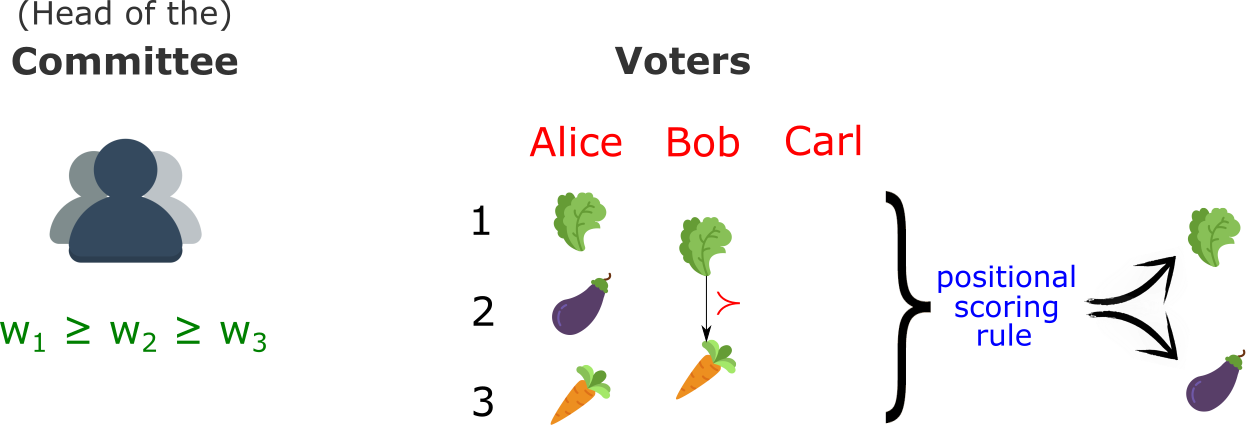
\includegraphics[scale=0.35]{set2.png}
%%		\caption{.}
%%		\label{fig:b1}
%	\end{figure}
%	\textbf{Goal}: Development of an incremental elicitation protocol based on minimax regret 
%\end{frame}

\subsection{Motivation and approach}
\begin{frame}
	\frametitle{Motivation and approach}
	\textbf{Who?}
	\begin{itemize}
		\item Imagine to be an \emph{external observer} helping with the voting procedure
	\end{itemize}
	\onslide<2-> \textbf{Why?}
	\begin{itemize}
		\item Voters: difficult or costly to order \emph{all} alternatives
		\item Committee: difficult to \emph{specify} a voting rule precisely and abstractly
	\end{itemize}
	\onslide<3-> \textbf{What?}
	\begin{itemize}
		\item We want to reduce uncertainty, inferring (\textit{eliciting}) the true preferences of voters and committee, in order to quickly converge to an optimal
		or a near-optimal alternative
	\end{itemize}		
\end{frame}

\begin{frame}
	\frametitle{Motivation and approach}
	\onslide<1-> \textbf{Approach}
	\begin{itemize}
		\item Develop query strategies that interleave questions to the committee and questions to the voters
		\item Use \emph{Minimax regret} to measure the quality of those strategies
	\end{itemize}
	\onslide<2-> \textbf{Assumptions}
	\begin{itemize}
		\item We consider \textit{positional scoring rules}, which attach weights to positions according to a scoring vector $w$
		\item We assume $w$ to be \textit{convex}
		\[ w_r - w_{r+1} \geq w_{r+1}-w_{r+2} \qquad \forall r\]
		and that $w_1=1$ and $w_m=0$
	\end{itemize}	
\end{frame}

\subsection{Related Works}
\begin{frame}
	\frametitle{Related Works}
	\textbf{Incomplete profile}  
	\begin{itemize}
		\item and known weights: Minimax regret to produce a robust winner approximation (\textit{Lu and Boutilier 2011}, \cite{Lu2011}; \textit{Boutilier et al. 2006}, \cite{Boutilier2006})
	\end{itemize}~\\
	\textbf{Uncertain weights} 
	\begin{itemize}
		\item and complete profile: dominance relations derived to eliminate alternatives always less preferred than others (\textit{Stein et al. 1994}, \cite{Stein1994})
		\item in positional scoring rules (\textit{Viappiani 2018}, \cite{Viappiani2018})
	\end{itemize}
\end{frame}

\subsection{Context}

\begin{frame}
	\frametitle{Context}

		\begin{description}[$W=(\w_k,\ 1\leq k \leq m), \ W \in \mathcal{W}$]
			\item [$A$] alternatives, $|A|=m$
			\item [$N$] voters 
			\item [$P = (\pref_j, \ j \in N ), \ P \in \mathcal{P} $] complete preferences profile 
			\item [$W=(\w_r,\ 1\leq r \leq m), \ W \in \mathcal{W}$] (convex) scoring vector that the committee has in mind
		\end{description}
		\bigskip
		\onslide<2-> \begin{block}{}
			$W$ defines a Positional Scoring Rule $f_W(P)\subseteq A$ using scores \color{blue}$s^{W,P}(a), \ \forall \ a \in A$
		\end{block}
		\onslide<3-> \begin{block}{}
			$P$ and $W$ exist in the minds of voters and committee but unknown to us
		\end{block}
		
\end{frame}

\subsection{Questions}
\begin{frame}
	\frametitle{Questions}
	\onslide<2-> \textbf{Questions to the voters}
	\begin{itemize}
		\item[] Comparison queries that ask a particular voter to compare two alternatives $a, b \in A$
		\color{blue}\[a \pref_j b \quad ?\]
	\end{itemize}
	\onslide<3->  \textbf{Questions to the committee}
	\begin{itemize}
		\item[] Queries relating the difference between the importance of consecutive ranks from $r$ to $r+2$
		\color{blue} \[ w_{r} - w_{r+1} \geq \lambda (w_{r+1} - w_{r+2}) \quad ? \] 
	\end{itemize}
\end{frame}

\subsection{Our Knowledge}
\begin{frame}
	\frametitle{Our Knowledge}
	The answers to these questions define $C_P$ and $C_W$ that is our knowledge about P and W 
	\medskip
	\begin{itemize}
		\onslide<2-> \item $C_P \subseteq \mathcal{P}$ constraints on the profile given by the voters
		\onslide<3-> \item $C_W \subseteq \mathcal{W}$ constraints on the voting rule given by the committee
	\end{itemize}
\end{frame}

\subsection{Definition}
\begin{frame}
	\frametitle{Minimax Regret}
	Given $C_P \subseteq \mathcal{P}$ and $C_W \subseteq \mathcal{W}$:
	
	\begin{block}{}
		\[\color{red}{\PMR^{C_P,C_W}(a,b)}= \max_{P\in C_P, W \in C_W} s^{P,W}(b)-s^{P,W}(a) \]
		is the maximum difference of score between $a$ and $b$ under all possible realizations of the full profile {\em and} weights
	\end{block}
	
	\onslide<2->  We care about the worst case loss: \emph{maximal regret} between a chosen alternative $a$ and best real alternative $b$
	\[\MR^{C_P,C_W}(a)= \max_{b\in A} \PMR^{C_P,C_W}(a,b) \]
	 	
	\onslide<3-> \centerline{\textbf{We select the alternative which \emph{minimizes} the maximal regret}}
	\[\MMR^{C_P,C_W}= \min_{a\in A} \MR^{C_P,C_W}(a)\]
\end{frame}

\subsection{Pairwise Max Regret Computation}
\begin{frame}
	\frametitle{Pairwise Max Regret Computation}
	The computation of $\PMR^{C_P,C_W}( \icimg{salad.png},\icimg{aubergine.png})$ can be seen as a game in which an adversary both:
	\begin{itemize}
		\onslide<2-> \item \textbf{chooses a complete profile $\mathbf{P \in \mathcal{P}}$}\\
		\medskip
		\begin{center}
			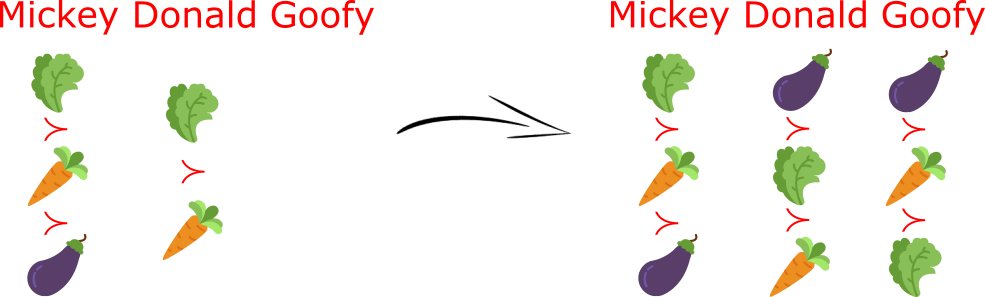
\includegraphics[scale=0.35]{completion4.png}
		\end{center}
		
		\onslide<3-> \item \textbf{chooses a feasible weight vector $\mathbf{W \in \mathcal{W}}$}\\
		\medskip
		\centerline{\color{red}$\mathbf{(1,?,0)}$ \icarr{arrow.png} \color{red}$\mathbf{(1,0,0)}$}
	\end{itemize}
	\medskip
	in order to maximize the difference of scores
\end{frame}

\subsection{Computing Minimax Regret}
\begin{frame}[t]
	\frametitle{Computing Minimax Regret: Example}
	\textbf{Profile completion}\\
	Consider the following partial profile
	\begin{center}
		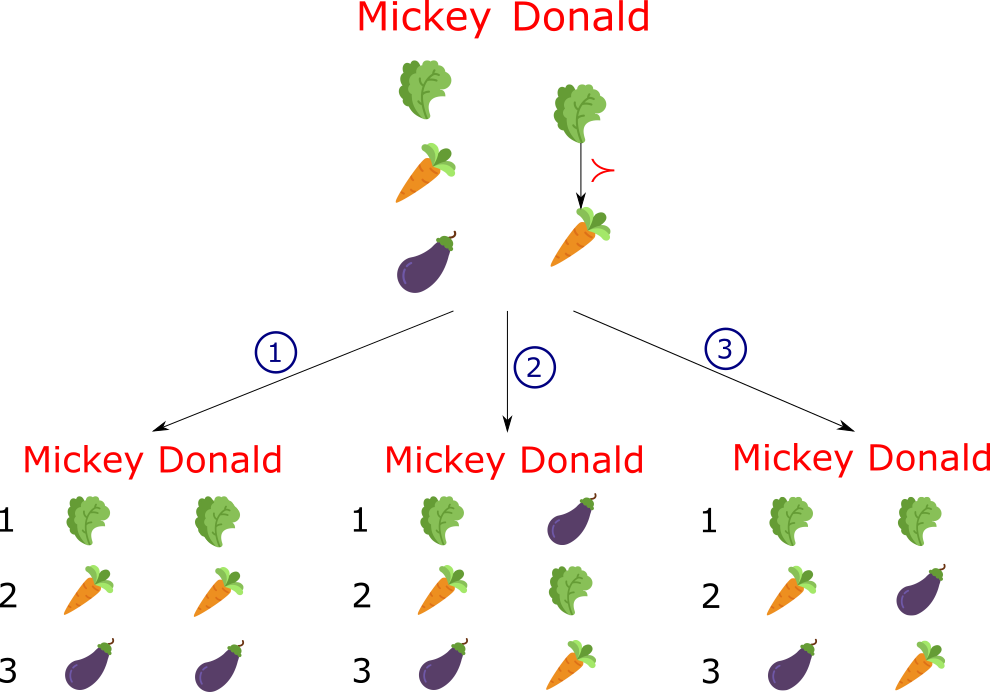
\includegraphics[scale=0.33]{compl.png}
	\end{center}
\end{frame}
\begin{frame}[t]
	\frametitle{Computing Minimax Regret: Example}
	\textbf{Weight selection} \\ \bigskip
	Consider the following constraint on the scoring vector given by the committee
	\[w_1 \geq 2 \cdot w_2\]
	and the convex assumption
	\[w_1 - w_2 \geq w_2 - w_3 \]

\end{frame}
\begin{frame}[t]
	\frametitle{Computing Minimax Regret: Example}
	\textbf{Minimax computing}\\
	\begin{center}
		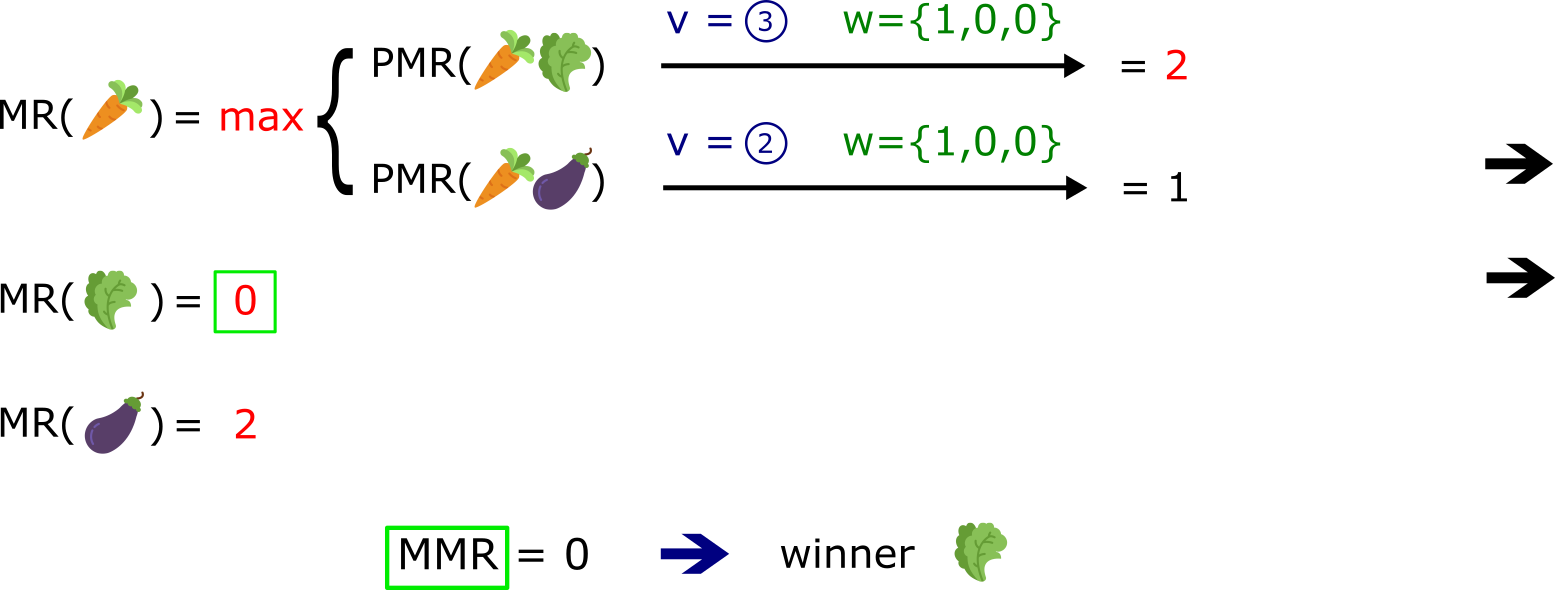
\includegraphics[scale=0.35]{minmax.png}
	\end{center}
\end{frame}

	
	\subsection{Elicitation strategies}
	\begin{frame}
		\frametitle{Elicitation strategies}
		At each step, the strategy selects a question to ask either to one of the voters about her preferences or to the committee about the voting rule \\ \bigskip
		\onslide<2-> The termination condition could be:
		\begin{itemize}
			\item <3-> when the minimax regret is lower than a threshold
			\item <4-> when the minimax regret is zero
		\end{itemize}
		\bigskip
	\end{frame}

	\begin{frame}[t]
		\frametitle{Elicitation strategies}
		\textbf{Random Strategy} \\
		\bigskip
		\onslide<2-> Decides with a probability of $\frac{1}{2}$ each whether to ask a question about
		\bigskip
			\begin{itemize}
				\item<3-> \textbf{weights}: it draws a rank $2 \leq r \leq m-2$ equiprobably, takes $\lambda$ as the middle of the interval of values we are still uncertain about, and asks whether $w_{r}-w_{r+1} \geq \lambda (w_{r+1} - w_{r+2})$
				\item<4-> \textbf{a preference ordering}: it draws equiprobably a voter whose preference is not known entirely and two alternatives that are incomparable in our current knowledge
			\end{itemize}
	\end{frame}	
	
	\begin{frame}[t]
		\frametitle{Elicitation strategies}
		\textbf{Pessimistic Strategy} \\
		\bigskip
		\onslide<2-> Assume that a question leads to the possible new knowledge states $(C_P^1, C_W^1)$ and $(C_P^2, C_W^2)$ depending on the answer, then the badness of the question in the worst case is:
		\[\max_{i=1,2} \MMR(C_P^i, C_W^i) \]
		\onslide<3-> The pessimistic strategy selects the question that leads to minimal regret in the worst case \\
		\bigskip
		\onslide<4-> \begin{block}{Note:}
			if the maximal MMR of two questions are equal, then prefers the one with the lowest MMR values associated to the opposite answer
		\end{block}
	\end{frame}	
	
	\begin{frame}[t]
		\frametitle{Elicitation strategies}
		\textbf{Two Phase Strategy} \\
		\bigskip
		\begin{itemize}
			\item <2-> \textbf{phase one:} asks a predefined sequence of $m - 2$ questions to the committee in order to gather informations about the weights (one per rank except the extremes)
			\item <3-> \textbf{phase two:} asks only questions to the voters, using the mechanism defined in the Pessimistic strategy
		\end{itemize}
	\end{frame}
	
	\begin{frame}[t]
		\frametitle{Elicitation strategies}
		\textbf{Extreme Completions Strategy} \\
		\medskip
		\onslide<2-> Let $a^{*}$ be the minimax regret optimal alternative, and $\bar{b}$, $\bar{P}$ and $\bar{W}$ the instantiations that maximize the regret when $a^*$ is chosen. \onslide<3-> Define: 
		\begin{align*}
		\tau_{W} & = \min_{W \in C_W} s^{\bar{P},W}(\bar{b}) - s^{\bar{P},W}(a^{*}) \\
		\tau_{P_i} & = \min_{\hat{P_i} \in C_P} s^{\hat{P_i},\bar{W}}(\bar{b}) -  s^{\hat{P_i},\bar{W}}(a^{*})
		\end{align*}
		where $\hat{P_i}$ is defined as $\bar{P}$ except for $i$ \\
		\bigskip
		\onslide<4->
		$\MMR - \tau_{W}$ estimates the contribution to the regret of our uncertainty about the weights; $\MMR - \tau_{P_i}$ estimates the uncertainty about the profile
		\\ \bigskip
		\onslide<5-> The extreme completions strategy asks a question to whoever minimizes $\tau$
	\end{frame}
	
	\subsection{Results}
	\begin{frame}
		\frametitle{Results}
		\sisetup{round-mode=places, round-precision=1, table-figures-integer=1, table-figures-decimal=1}
		\begin{table}
			\begin{center}
				\begin{tabular}{S[table-figures-integer=2, table-number-alignment = right, table-figures-decimal=0]S[table-number-alignment = right]@{$\pm$}S[table-number-alignment = left]S[table-number-alignment = right]@{$\pm$}S[table-number-alignment = left]S[table-number-alignment = right]@{$\pm$}S[table-number-alignment = left]S[table-number-alignment = right]@{$\pm$}S[table-number-alignment = left]}
					\hline
					{k} & {Rnd} & {sd} & {T. ph.} & {sd} & {Pes.} & {sd} \\
					\hline
					0 & 5.0 & 0 & 5.0 & 0 & 5.0 & 0\\
					5 & 4.93 & 0.16 & 4.98 & 0.01 & 4.15 & 0.32\\
					10 & 4.84 & 0.22 & 4.35 & 0.28 & 3.44 & 0.46\\
					15 & 4.28 & 0.58 & 3.70 & 0.25 & 2.66 &0.54 \\
					20 & 3.85 & 0.33 & 2.67 & 0.51 & 1.62 & 0.82\\
					25 & 3.50 & 0.78 & 2.17 & 0.66 & 0.84 &  0.57\\
					30 & 2.96 & 0.80 & 1.47 & 1.10 & 0.53 & 0.70\\
					\hline
				\end{tabular}
			\end{center}
			\caption{Minimax regret in problems of size $(5, 5)$ after $k$ questions.}
			\label{fig:xp2}
		\end{table}
	\end{frame}

\section{Preference Elicitation under Majority Judgment}

\addtocounter{framenumber}{-1}
\begin{frame}[plain]
	\centering \color{darkred}\LARGE Thank You!
\end{frame}




\bibliographystyle{plain}
\bibliography{biblio} 
%given a combination of axioms we want to find an outcome that doesn't satisfy them, and we would do that for several reasons:
%-querying the user, depending of her answer we might infer her preferences over the set of axioms;
%-proving that a set of axioms is not valid giving a counter-example;


%A method for automatically proving impossibility theorems in the area of ranking sets of objects has already been implemented (Geist \& Endriss, 2011). It:



\end{document}